\section{Pose Refinement with Learned Depth Maps}

\label{sec:method}

\begin{frame}{Method overview}
	\only<1>{
		\begin{figure}
		\centering		
		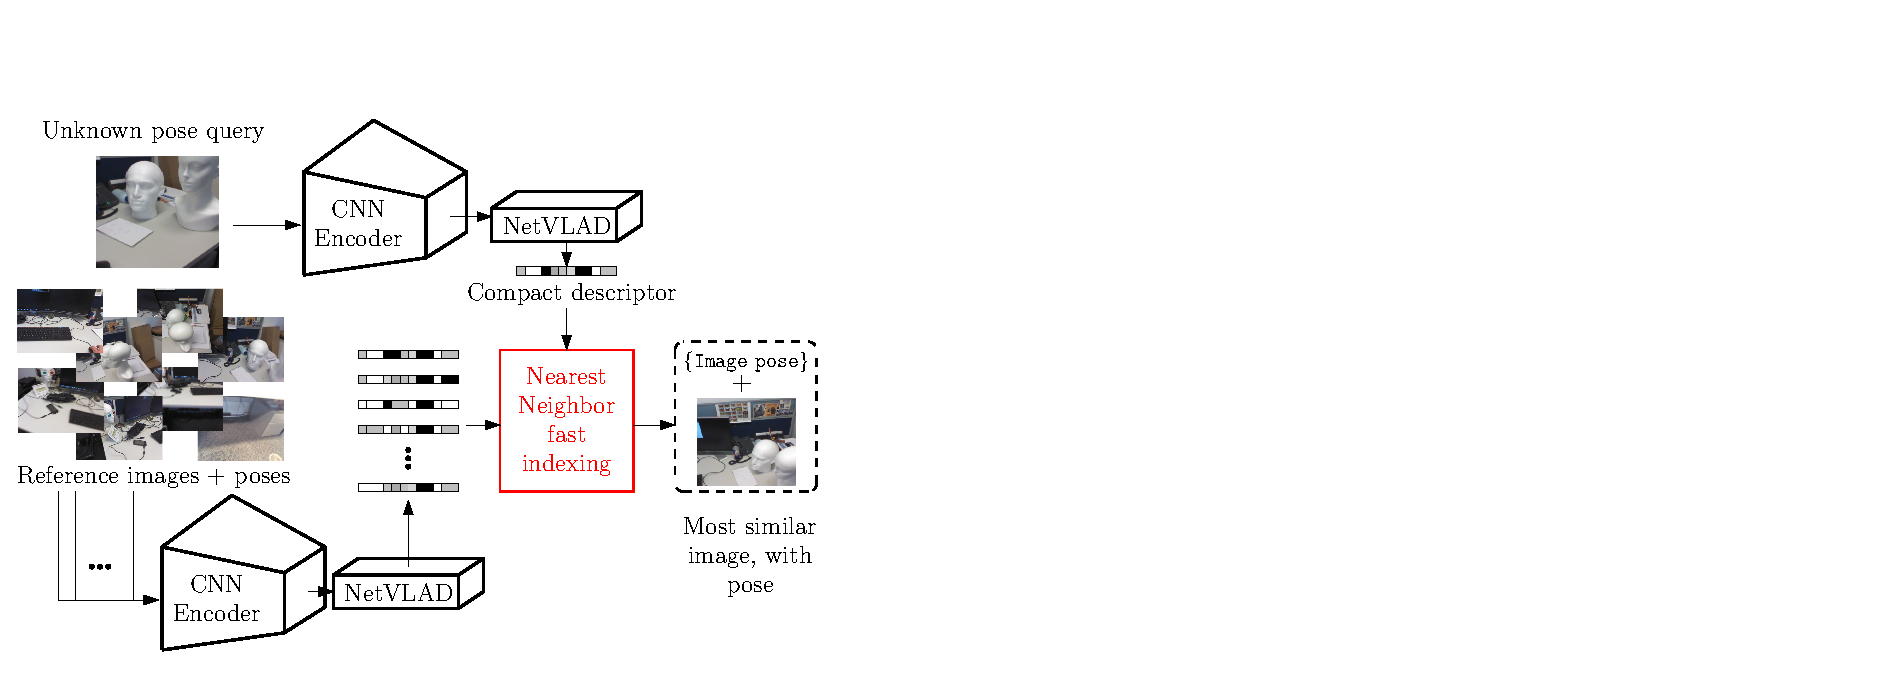
\includegraphics[width=0.9\linewidth]{images/method/1}
		\end{figure}
		
		\vfill
		
		Initial pose obtained by image retrieval.
	}
	\only<2>
	{
		\begin{figure}
		\centering
		\includegraphics[width=0.9\linewidth]{images/method/2}
		\end{figure}	
		
		\vfill
		
		Dense correspondences are made by matching CNN deep features.
	}
	\only<3>
	{
		\begin{figure}
		\centering
		\includegraphics[width=0.9\linewidth]{images/method/3}
		\end{figure}	
		
		\vfill
	
		\textbf{Method 1)} Initial approach: projection of the matched 2D points according to the produced depth map and alignment of the obtained 3D points clouds by ICP.
	}
	\only<4>
	{
		\begin{figure}
		\centering
		\includegraphics[width=0.9\linewidth]{images/method/4}
		\end{figure}	
		
		\vfill
	
		\textbf{Method 2)} Minimising the depth incertitude: pose estimation by Perspective-n-Point (PnlP).
	}
\end{frame}

\begin{frame}{Method details}
	Dense local correspondences:
	\begin{itemize}
		\item feature block with same spatial dimension as depth output (2nd conv. block)
		\item bidirectional matching
	\end{itemize}

	\vfill	
	
	\uncover<2>
	{
	Pose estimation:
	\begin{itemize}
		\item ICP and PnP optimization within RANSAC
		\item we evaluate the top 5 retrieved candidates from the image retrieval first step
	\end{itemize}
	}
\end{frame}

\begin{frame}{System design and motivation}
	\begin{block}{Multi-task model}
		Same network for: global image description, dense local feature matching and depth from monocular.
	\end{block}
	\vfill
	\uncover<2->
	{
		\begin{block}{Single task training policy}
			We decide to train our network for the task of depth from monocular because erroneous depth estimation measurement will result in wrong estimation of the final pose.
		\end{block}
	}
	\vfill
	\uncover<3>
	{
		\begin{block}{Generalisation}
			The same trained network can be used to localise images in multiple indoor and outdoor scenes, and even on totally unknown environments.
		\end{block}
	}
\end{frame}

